\section{Background and Motivation}

In this section, we first briefly introduce baseline systolic arrays and how
they perform matrix multiplications. We then present the \FA{} algorithm and
discuss inefficiencies of running it on systolic arrays.
Finally, we motivate the approach of fusing the entire \FA{} on a single systolic array.

\subsection{Matrix Multiplication on Systolic Arrays}\label{sec:systolic-array-intro}

Systolic arrays are a class of architectures where data flows through an array of processing elements (PEs) in a rhythmic fashion.
\autoref{fig:systolic-array-example} depicts the basic structure of a systolic array,
comprising $N \times N$ PEs forming a two-dimensional array.
Each PE performs one simple arithmetic operation, such as multiply-accumulate (MAC),
on its input, and drives the output to the next PE, dictated by the array's dataflow.
According to what data is reused in the computation, the dataflow can be categorized as 
\emph{weight-stationary}, \emph{input-stationary}, \emph{output-stationary}, 
or \emph{row-stationary}~\cite{eyeriss-isca}.
As most deep learning workloads favor weight reuse,
many systolic-array-based accelerators,
including Google's TPU~\cite{google-tpu-arch}, adopt the weight-stationary dataflow.

\begin{figure}[t]
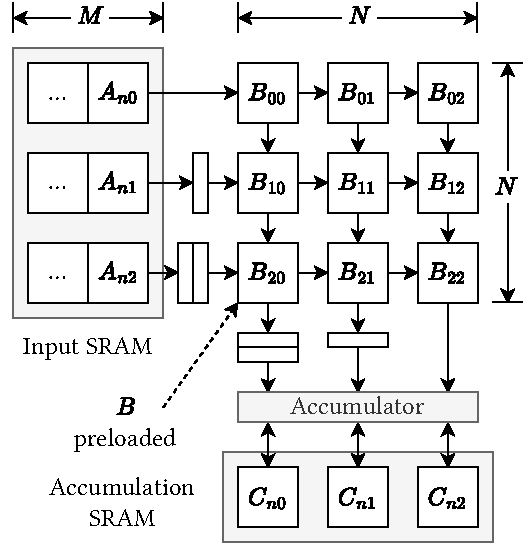
\includegraphics[scale=0.75]{figure_src/sa.drawio.pdf}
\caption{Computing $C \mathrel{+}= AB$ on a weight-stationary systolic array.}
\label{fig:systolic-array-example}
\Description{SA}
\end{figure}

Matrix operations, especially matrix multiplication,
are particularly well-suited for systolic arrays because of their high regularity of computation.
To perform matrix multiplication $C \mathrel{+}= A B$ on a weight-stationary systolic array,
the weight matrix $B$ is preloaded into the array,
while the input matrix $A$, shaped as $M \times N$,
is streamed in from an input SRAM.
To ensure correctness, each row of the input matrix must be delayed by $0$ to $N-1$ cycles
before entering the array. Consequently, each column of the output matrix must be delayed
by $0$ to $N-1$ cycles before use.
The systolic array does not save the output matrix $C$ itself.
Instead, the output matrix is stored in a separate \emph{Accumulation SRAM}
located at the bottom of the array.
The \emph{Accumulator} reads the old values of $C$ from the SRAM,
merges them with the systolic array's output,
and writes the merged values back to the accumulation SRAM.
This near-memory accumulation scheme is widely adopted in both open-source accelerators~\cite{ucb-gemmini}
and commercial products~\cite{trainium-arch}.

During the entire matrix multiplication, MAC computation consumes $M$ cycles,
while weight matrix preloading takes $N$ cycles,
and delaying the input rows and output columns takes another $2 N - 1$ cycles.
In total, the entire computation takes $M + 3N - 1$ cycles to finish,
resulting in a theoretical array utilization of $M / (M + 3N - 1)$. 
When $M \gg N$, the data preparation overhead is negligible.


\subsection{\FA{} on Systolic Arrays}\label{sec:fa-algorithm}

\SetKwInput{kwRequire}{Require}
\tikzHighLight{mat1}{LightSalmon}{{-0.5em, 1em}}{{10em, -0.5em}}
\tikzHighLight{vec}{RoyalBlue}{{-0.5em, 1em}}{{5.7em, -0.5em}}
\tikzHighLight{mat2}{LightSalmon}{{-0.5em, 0.9em}}{{9.05em, -1.7em}}
\begin{algorithm}[t]
    \caption{\FA{}-2 and 3 forward pass}
    \label{alg:flash-attention}
    \kwRequire{Matrices $Q, K, V \in \mathbb{R}^{LEN \times d}$}
    Divide $Q$ into $T_{r} = \lceil \frac{LEN}{B_{r}} \rceil$ blocks of size $B_{r} \times d$ each,
    and divide $K$ and $V$ into $T_{c} = \lceil \frac{LEN}{B_{c}} \rceil$ blocks of size $B_{c} \times d$ each\;
    \For {$ 1 \leq i \leq T_{r} $}
    {
        Initialize $old_m, old_l = (-\infty), (0) \in \mathbb{R}^{B_{r}} $\;
        Initialize $old_O = (0) \in \mathbb{R}^{B_{r} \times d} $\;
        \For {$ 1 \leq j \leq T_{c} $}
        {
            \tikzmark{mat1-start}$ S = Q_{i}K_{j}^{T} \in \mathbb{R}^{B_{r} \times B_{c}} $\tikzmark{mat1-end}\; \label{line:mat1}
            \tikzmark{vec-start}$ local_m = rowmax(S) \in \mathbb{R}^{B_{r}} $\; \label{line:rowmax-start}
            $ new_m = max(local_m, old_m) \in \mathbb{R}^{B_{r}} $\; \label{line:new-m}
            $ a = old_m - new_m \in \mathbb{R}^{B_{r}} $\; \label{line:rowmax-end}
            $ b = exp(\frac{a}{\sqrt{d}}) = exp2(\frac{\log_2 e}{\sqrt{d}}a) \in \mathbb{R}^{B_{r}} $\;
            $ N = S - new_m \in \mathbb{R}^{B_{r} \times B_{c}} $\; \label{line:s-minus-rowmax}
            $ P = exp(\frac{N}{\sqrt{d}}) = exp2(\frac{\log_2 e}{\sqrt{d}}N) \in \mathbb{R}^{B_{r} \times B_{c}} $\; \label{line:exp}
            $ local_l = rowsum(P) \in \mathbb{R}^{B_{r}} $\; \label{line:rowsum}
            $ new_l = old_l \times b + local_l \in \mathbb{R}^{B_{r}} $\tikzmark{vec-end}\; \label{line:l-acc}
            \tikzmark{mat2-start}$ local_O = PV_{j} \in \mathbb{R}^{B_{r} \times d} $\tikzmark{mat2-end}\; \label{line:mat2}
            $ new_O = diag(b)old_O + local_O \in \mathbb{R}^{B_{r} \times d} $\; \label{line:O-acc}
            $ old_m = new_m $\;
            $ old_l = new_l $\;
            $ old_O = new_O $\;
        }
        $ O_{i} = diag(old_l)^{-1}old_O \in \mathbb{R}^{B_{r} \times d} $\; \label{line:re-scaling}
    }
\end{algorithm}

\FA{}~\cite{fa2,fa3} is a memory-efficient attention algorithm that addresses the quadratic memory complexity bottleneck
of standard attention mechanisms.
\FA{} reformulates the attention calculation with tiling and online-softmax to reduce memory usage,
enabling the process of much longer sequences on hardware accelerators with limited on-chip storage.
The \FA{} algorithm is shown in \autoref{alg:flash-attention}.
Same as the official open-source \FA{} implementation~\cite{fa2},
the \texttt{exp} function is implemented as $\exp(x) = 2^{x \log_2 e}$ to benefit from the more
efficient \texttt{exp2} implementation in hardware~\cite{hwexp2}.

\FA{} contains two matrix multiplications (highlighted in red) and various non-matrix-multiplication operations in between,
such as reductions and element-wise computations for softmax (highlighted in blue).
When running \FA{} on systolic-array-based accelerators, the two matrix multiplications are executed on the systolic array,
while other softmax-related operations are offloaded to external vector or scalar units~\cite{trainium-arch}.
This simplistic mapping of computation forces intermediate results to be transferred back and forth between
the systolic array and vector/scalar units through a local SRAM,
essentially destroying any overlap and data reuse between the two matrix multiplications and exaggerating SRAM port contention~\cite{virgo,mosaic}.

To amortize this data movement overhead,
software usually incorporates large tile sizes and schedules multiple Flash\-Attention iterations in a pipelined manner.
However, due to the simplistic mapping of computation with matrix multiplication to the systolic array and softmax to vector/scalar units,
achieving high performance for \FA{} remains challenging~\cite{fusemax},
especially under the silicon constraint that prevents vector/scalar units from providing sufficient \FLOPs{}
to keep up with the systolic array.

\subsection{Fusing \FA{} into Systolic Arrays}

A possible approach to both eliminate the above data movement overhead and improve computation mapping is to discard vector/scalar units and run the entire \FA{} solely on the systolic array.
In this approach, no intermediate results need to be transferred,
and non-matrix-multiplication operations can utilize and share the abundant \FLOPs{} from the systolic array with matrix multiplication,
thereby significantly improving overall hardware utilization.

While seemingly straightforward,
this approach faces the practical challenge of implementing reduction or element-wise operations,
such as \texttt{exp}, \texttt{rowsum}, and \texttt{rowmax}, on the systolic array.
Such implementation is not trivial, as non-linear operations are not a natural fit for systolic arrays.
An efficient implementation without excessively extending the systolic array's PEs or dataflow requires
careful analysis of the arithmetic properties of these operations and novel extensions to the baseline systolic array architecture.
In addition, the numerical accuracy of these operations must be carefully handled to maintain correctness.

Fusing the entire \FA{} into a single systolic array gives us the extra benefit of overlapping executions
of matrix multiplications and softmax operations to further improve hardware utilization.
Similarly, all intermediate results can be generated and consumed in place without resorting to external SRAMs to eliminate SRAM port contention.
Both of these benefits can only be obtained through efficient and fine-grained scheduling of operations in \FA{}.
